\chapter{Experimental Tasks}

Before the tasks were performed the PIN diode was set into the test set-up. Therefore it was aligned into the optical path of the laser. To align the diode the laser was driven at a constant laser current. The position of diode was adjusted to maximize the photo current. 


Beside the laser light the diode detected extraneous light as well. This leads to an offset of the measured photo current. With the laser switched off a photo current varying between 2.2 and 2.4~$\upmu$A could be measured.

\section{Task 1: Field characteristic of a PIN diode I}
\label{T1}
\begin{figure}%
\centering
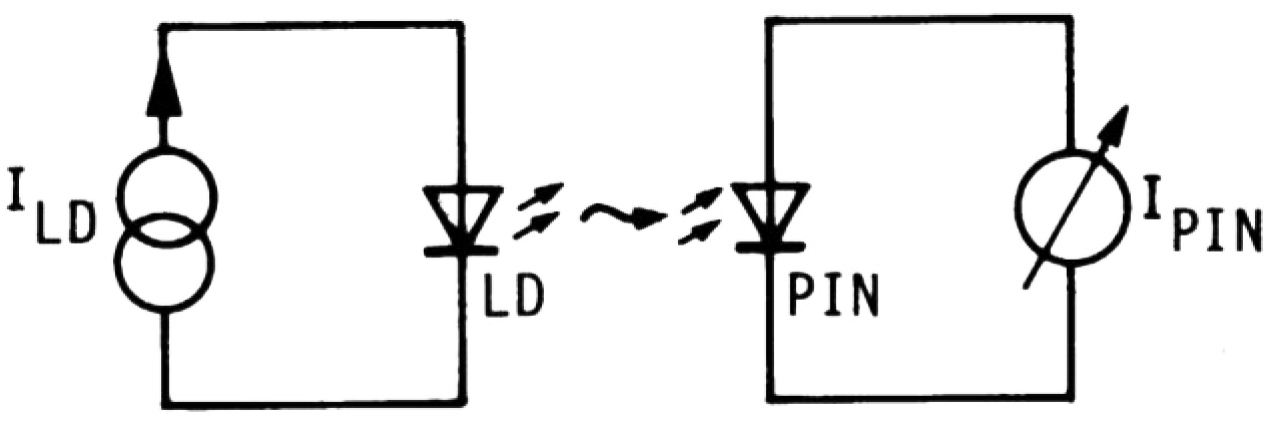
\includegraphics[width=.5\columnwidth]{Grafiken/T1_setup.jpg}%
\caption{Setup task 1}%
\label{fig:T1_setup}%
\end{figure}
In this task the short-circuit current $I_{\mathrm{PIN}}$ of the PIN diode was measured for different laser currents. Figure \ref{fig:T1_setup}\footnotemark[3] shows the used setup. 

The laser current was swept from 0 to 60~mA. In the range from 0 to 10~mA a step size of the current change of 0.4~mA was used. From 10 to 20~mA the step size was 1~mA and from 20 to 60~mA a stepsize of 5~mA was used. 

\begin{figure}%
\centering
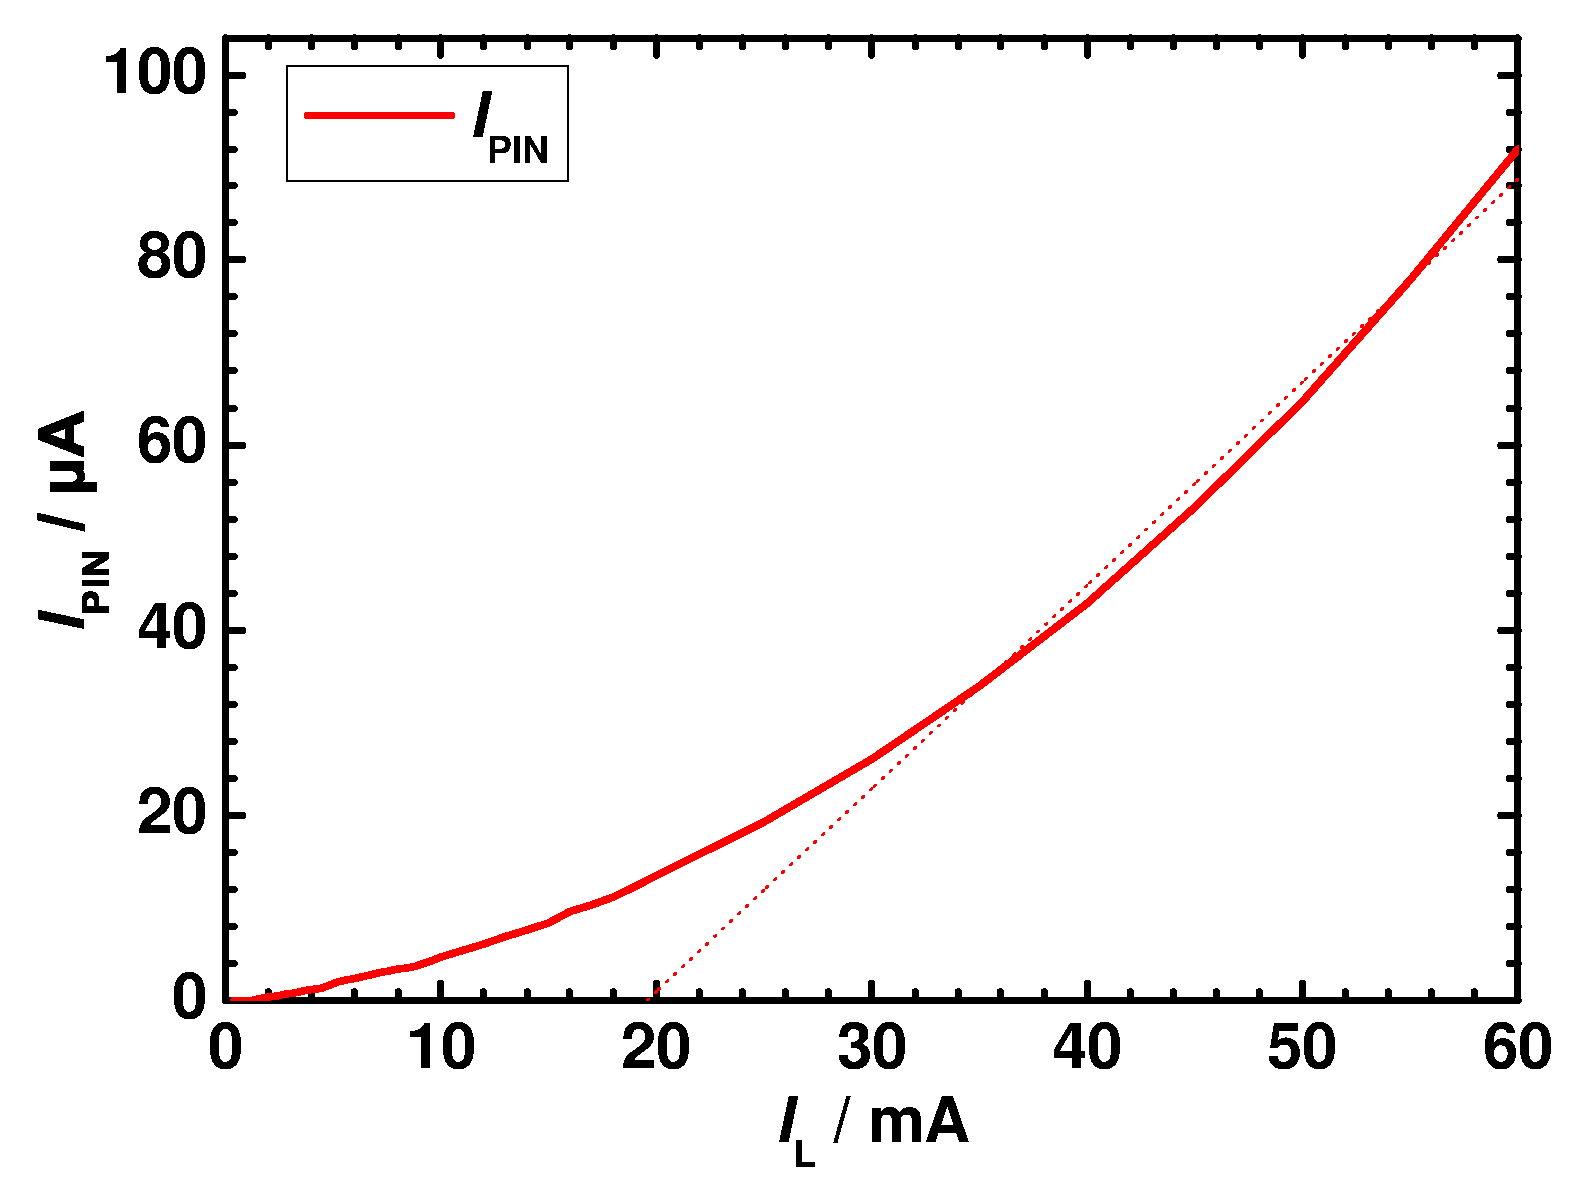
\includegraphics[width=.5\columnwidth]{Grafiken/T1_laser.pdf}%
\caption{Measured short-circuit currents.}%
\label{fig:T1_laser}%
\end{figure}

Figure \ref{fig:T1_laser} shows the measured short-circuit current $I_{\mathrm{PIN}}$ as a function of the laser current $I_{\mathrm{L}}$. The values of $I_{\mathrm{PIN}}$ are adjusted by 2.2~$\upmu$A. Thereby the value for the laser in off-state is 0~$\upmu$A.

Due to the fact that the measurement was not performed in a dark environment, the ambient light had impact on the measurements. To approximate the threshold a linear dependence of the number of photons emitted by the laser diode and the laser current was assumed \footnotemark[1]. Since the power depends of the number of photons and the photo current is proportional to the laser power, the connection between $I_{\mathrm{PIN}}$ and $I_{\mathrm{L}}$ can be assumed as linear as well. The linear emission should start at the threshold current. Because of spontaneous emission in the laser diode the emission starts below this threshold.

To approximate the threshold a linear fitting of the curve was performed. Only values of $I_{\mathrm{L}} \geq 30$~mA were taken into account because the spontaneous emission is of no consequence there. Figure \ref{fig:T1_laser} shows the linear fit as well. The intercept with $I_{\mathrm{PIN}} = 0~\upmu$A is at $I_{\mathrm{th}} \approx 20$mA. This can be assumed as the threshold of the laser diode.



For the next tasks four laser currents were selected. The corresponding photo currents are equidistant. Table \ref{tab:T1_values} shows the selected currents. Since the photo current is proportional to the incoming radiant power, the corresponding powers at the four laser currents are equidistant as well.


\begin{table}%
\centering
\caption{Laser currents and corresponding photo currents.}

\begin{tabular}{cc}

\toprule
$I_{\mathrm{L}}$ / mA	&	$I_{\mathrm{PIN}}$ / $\upmu$A\\

\midrule

19.5&15.0\\
31.4&30.0\\
40.0&45.0\\
47.1&60.0\\
\bottomrule 
\end{tabular}
\label{tab:T1_values}
\end{table}

\section{Task 2: Field characteristic of a PIN diode II}

In the second task first a bias is applied to the PIN-diode (cf. \ref{fig:T2_setup}). The voltage is varied from 0.1~V to 0.6~V and the $I_{\mathrm{PIN}}$ is recorded for the four $I_{\mathrm{pr}}$ determined in the first task (cf tabular \ref{tab:T1_values}). The voltage $U_{\mathrm{PIN0}} = U_{\mathrm{PIN}}(I_{\mathrm{PIN}}=0)$ is determined as well. Figure \ref{fig:UPIN0} shows the dependency of $\exp(U_{\mathrm{PIN0}}/U_{\mathrm{T}})$ on $I_{\mathrm{pr}}$.

 


\begin{figure}%
\centering
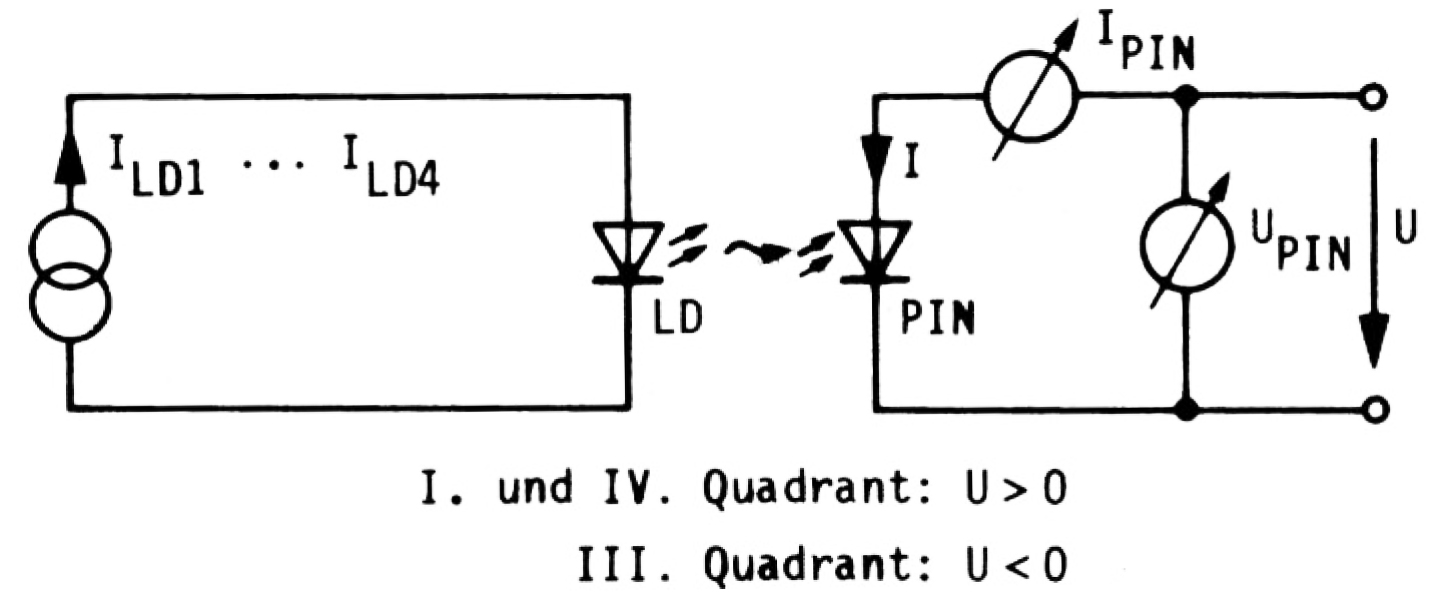
\includegraphics[width=.6\columnwidth]{Grafiken/T2_setup.jpg}%
\caption{}%
\label{fig:T2_setup}%
\end{figure}

\begin{figure}%
\centering
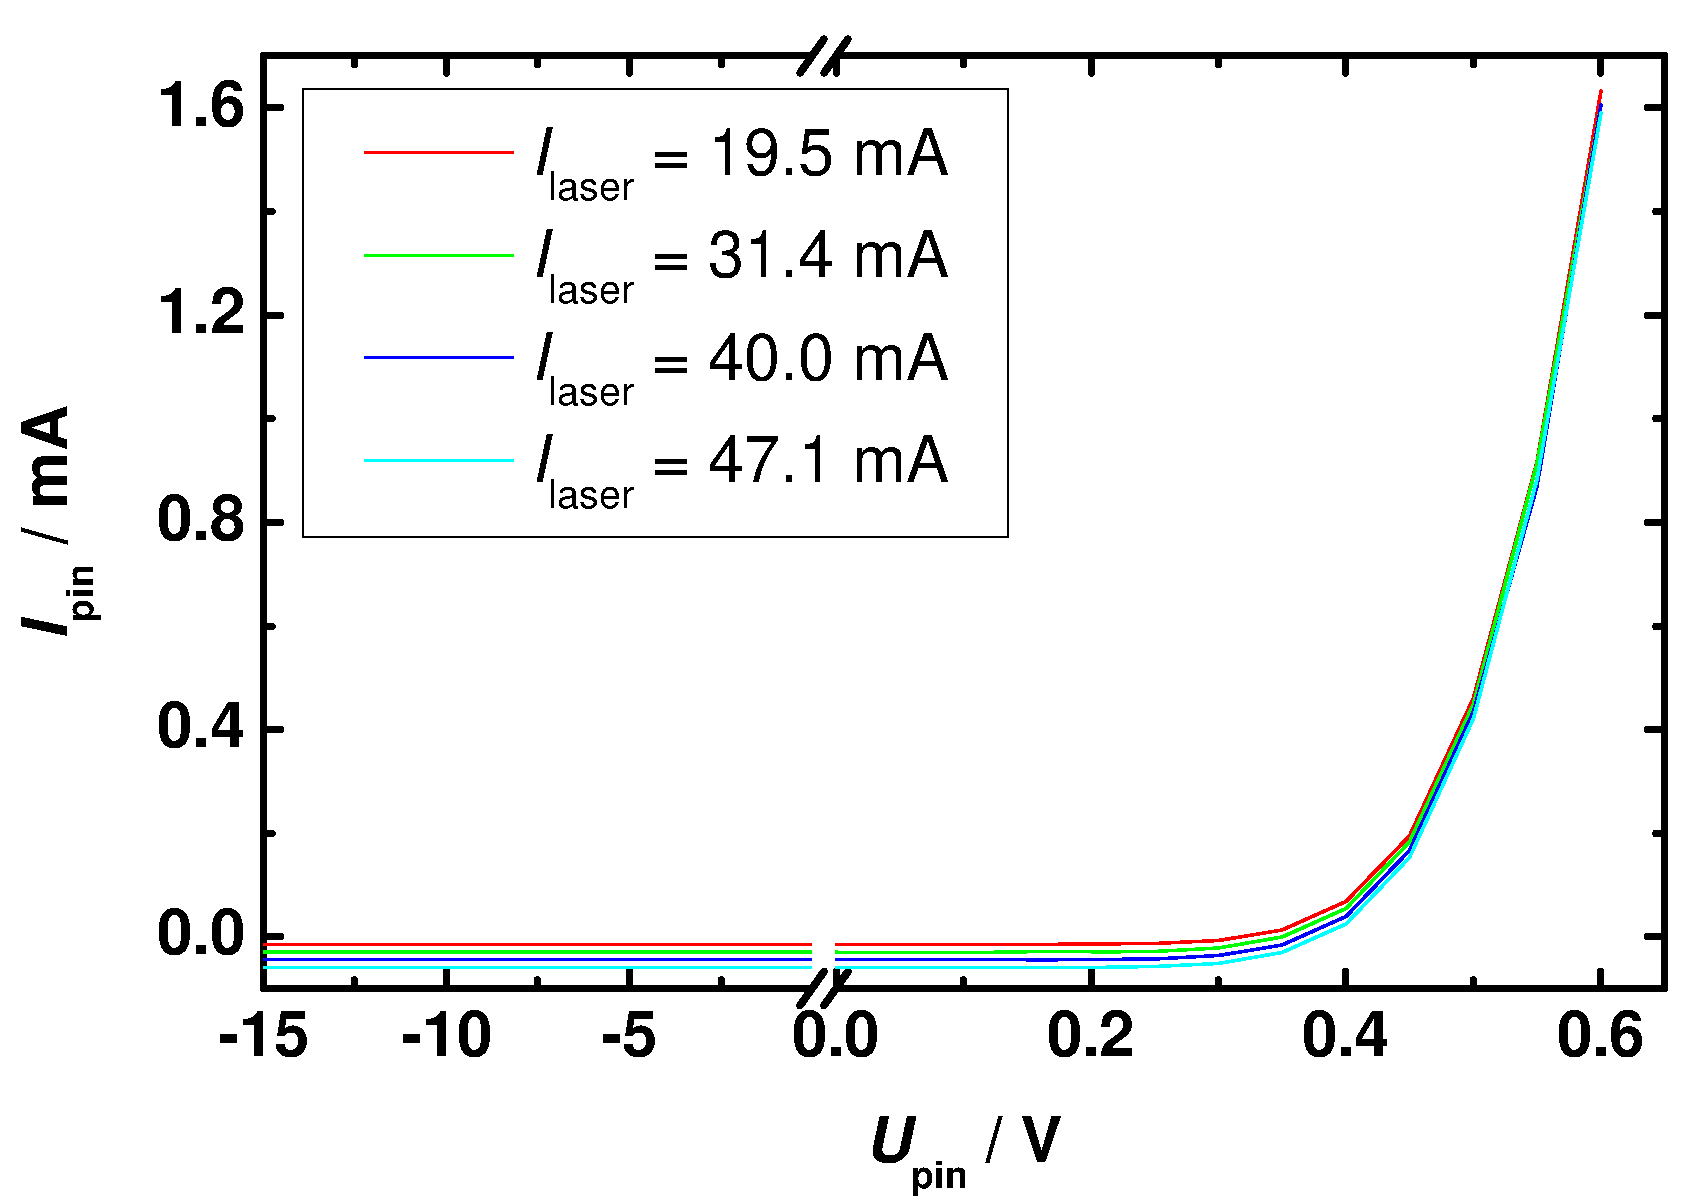
\includegraphics[width=.6\columnwidth]{Grafiken/PIN_kombiniert.pdf}%
\caption{}%
\label{fig:PIN_kombiniert}%
\end{figure}
\begin{figure}%
\centering
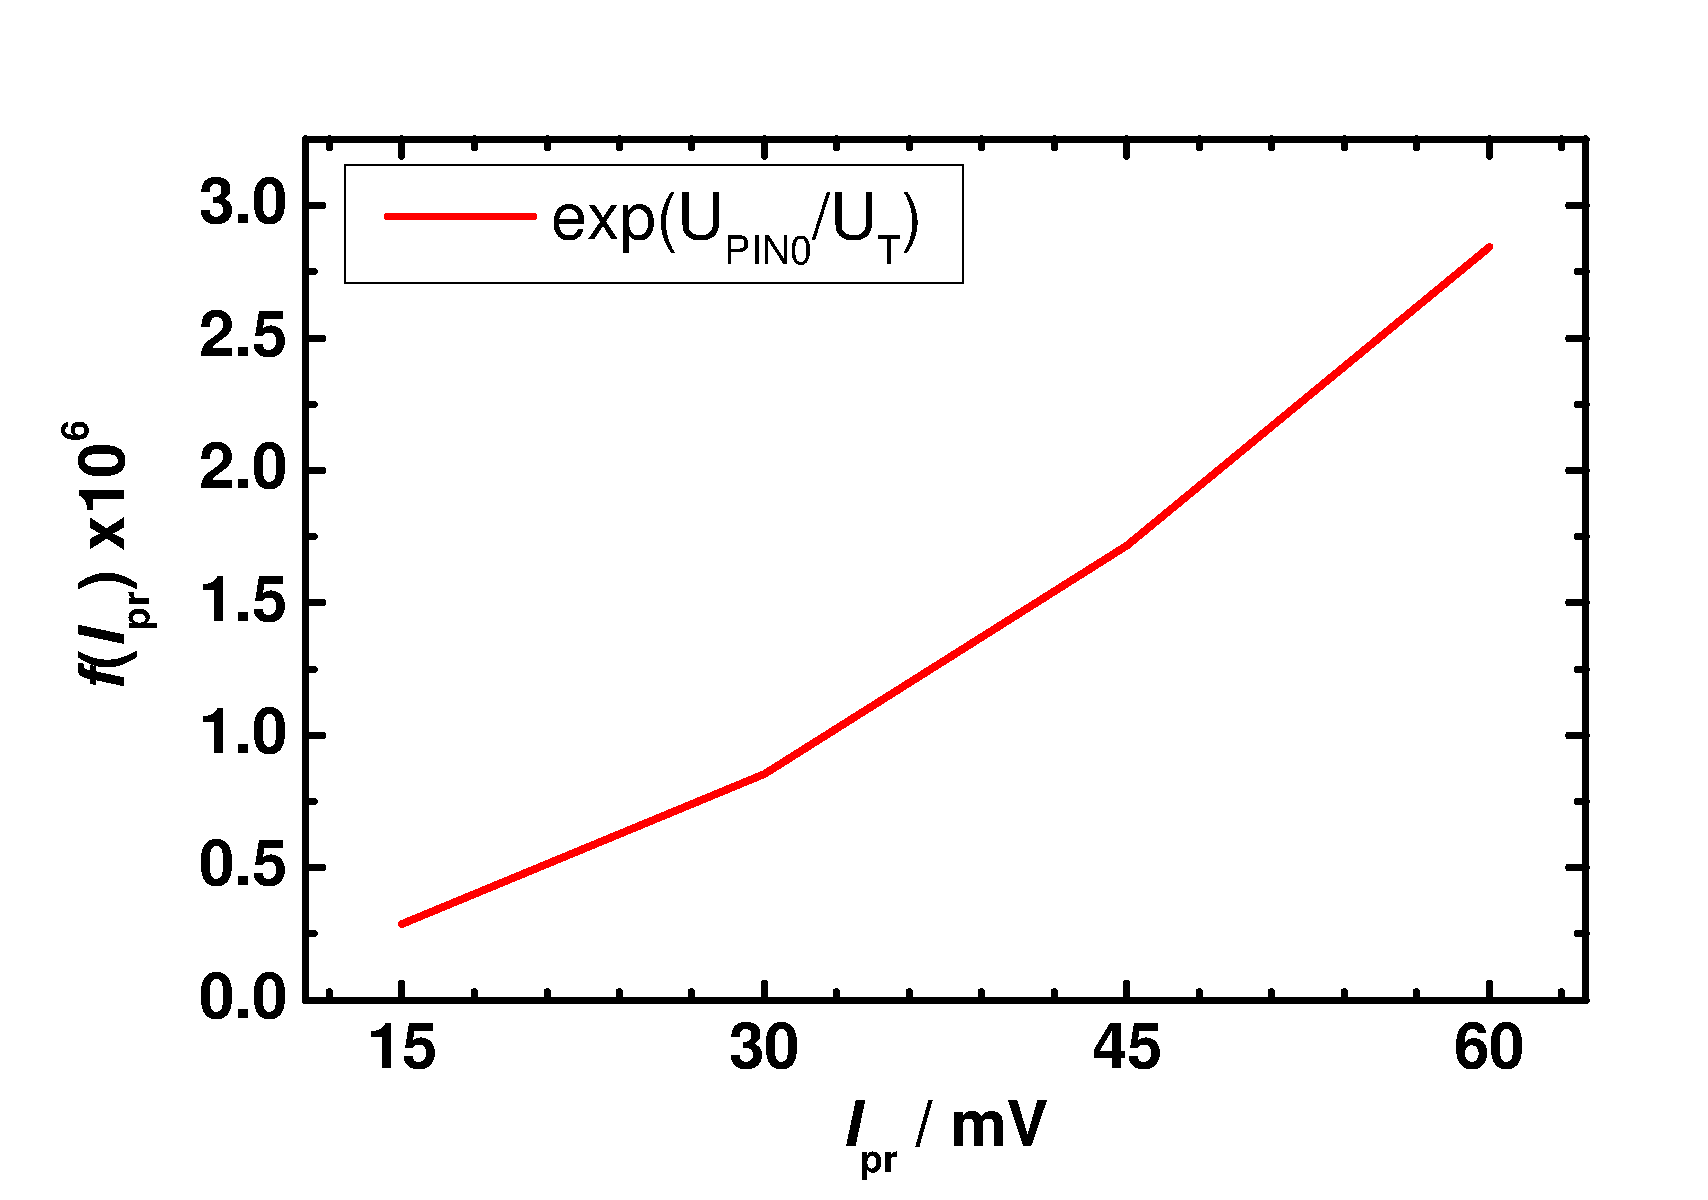
\includegraphics[width=.6\columnwidth]{Grafiken/UPIN0.pdf}%
\caption{}%
\label{fig:UPIN0}%
\end{figure}

\section{Task 3: Field characteristic of an APD}

For this task a APD was integrated into the setup. The diode was aligned to maximize the output current $I_{\mathrm{APD}}$.
Figure \ref{fig:T3_setup}\footnotemark[3] shows the setup.

To measure the caracteristic of the laser diode a reverse voltage ov $U = -10$~V was applied to the APD and the series resistance $R_{\mathrm{V}}$. "The voltage corresponds to an avalanche multiplication factor $M_0 \approx 1$"\footnotemark[3].

\begin{figure}%
\centering
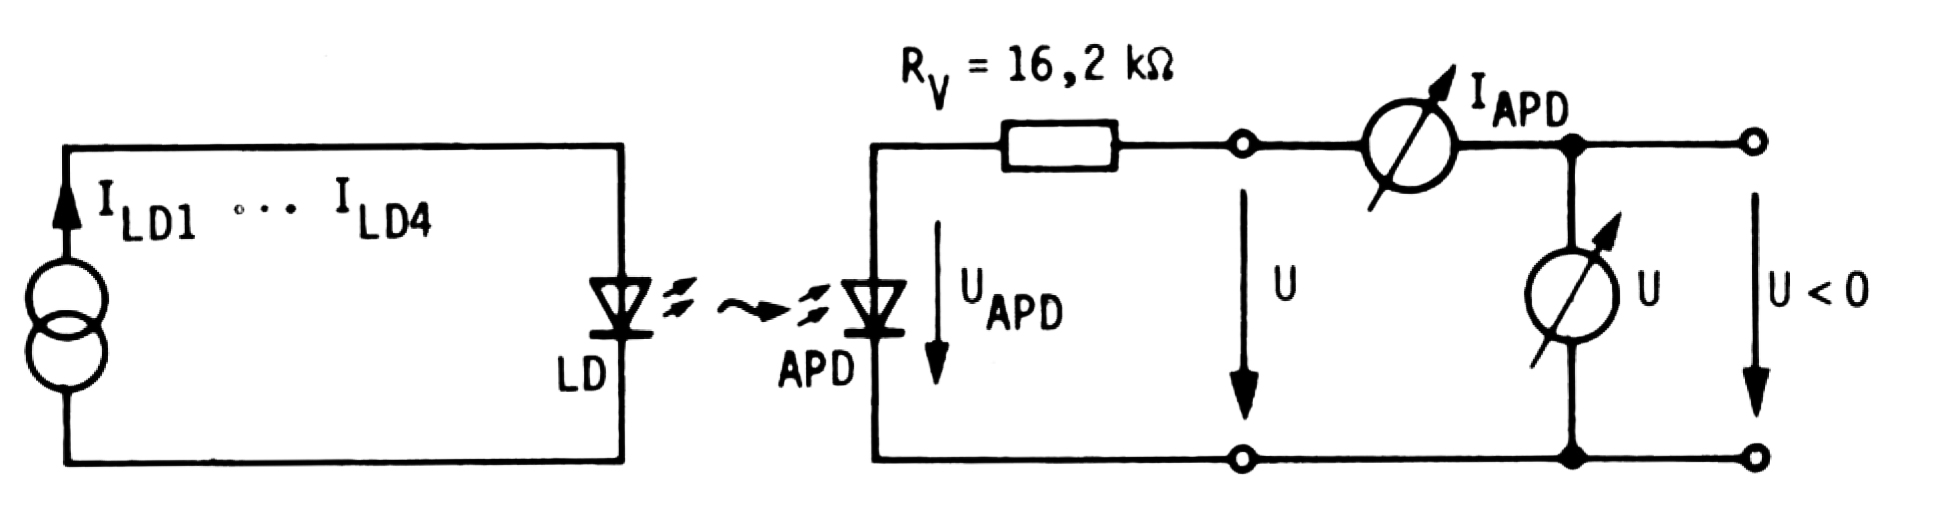
\includegraphics[width=.85\columnwidth]{Grafiken/T3_setup.jpg}%
\caption{}%
\label{fig:T3_setup}%
\end{figure}


\begin{figure}%
\centering
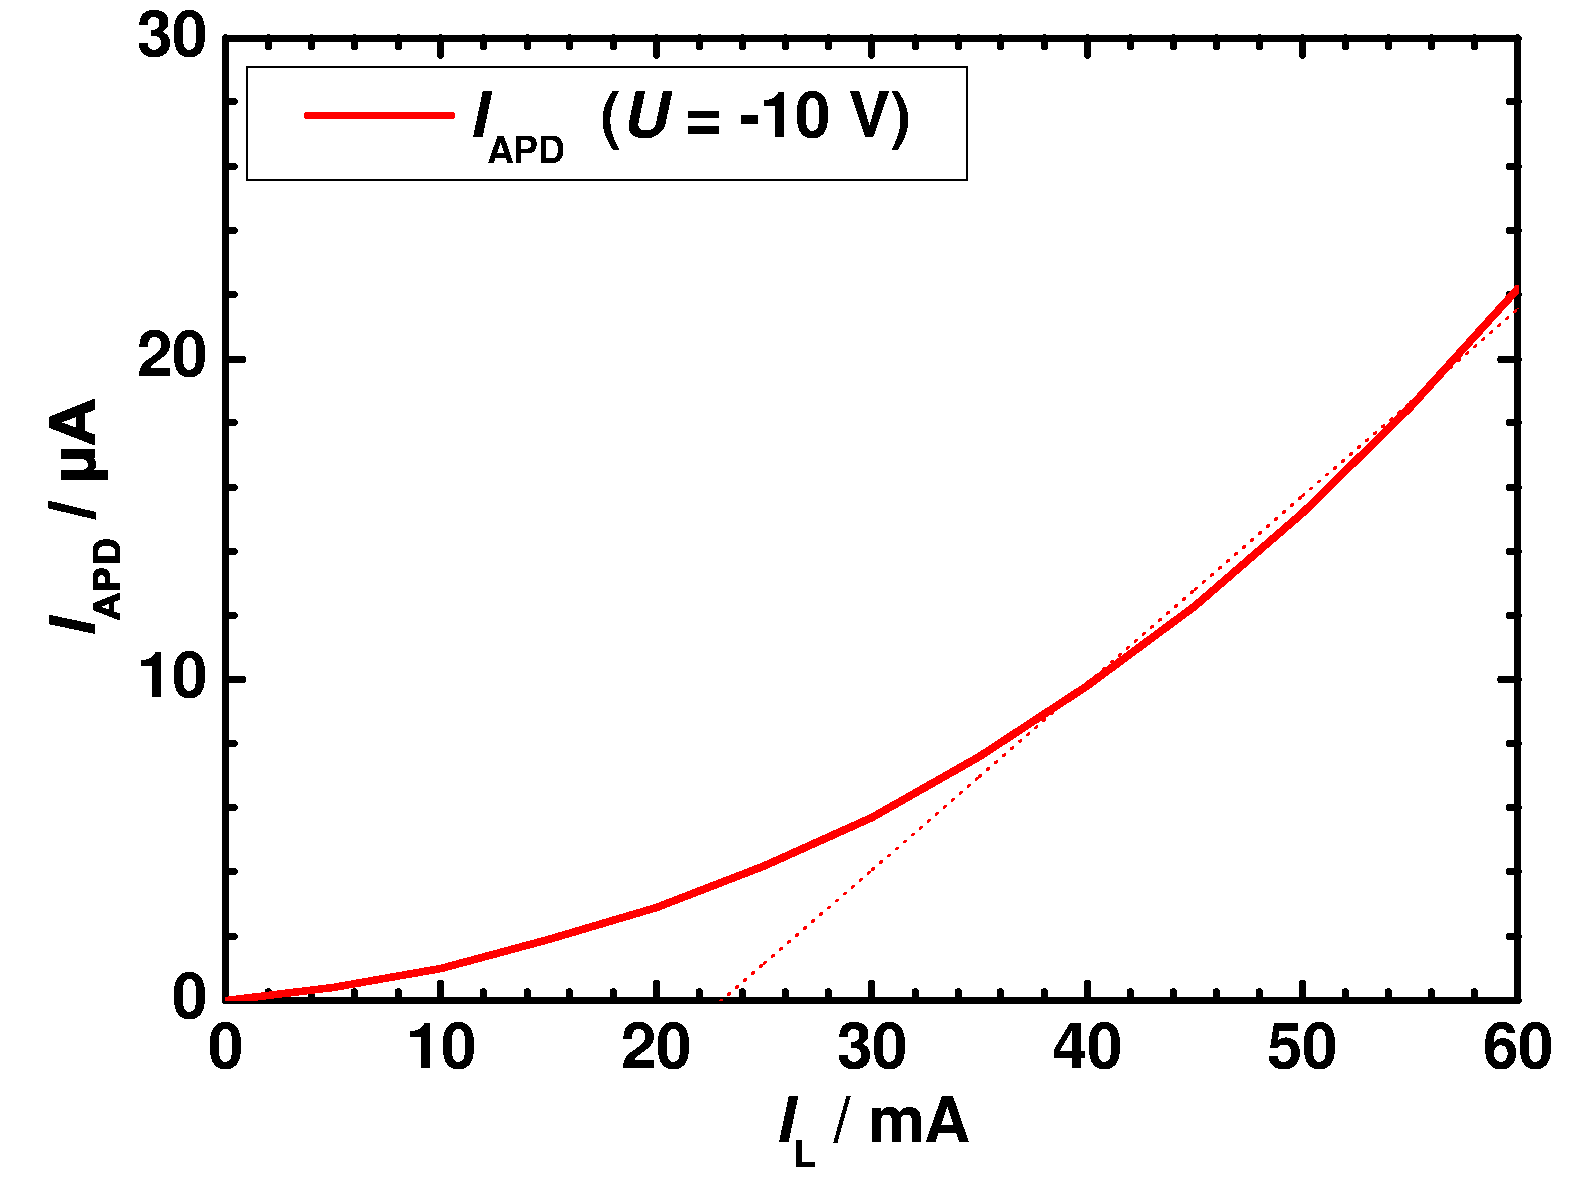
\includegraphics[width=.5\columnwidth]{Grafiken/T3_laser.pdf}%
\caption{Dependency of the photo current of the APD on the laser current.}%
\label{fig:T3_laser}%
\end{figure}


A laser current range from 0~mA~$\leq I_{\mathrm{L}} \leq 60$~mA was swept in 5~mA steps. There was no offset of $I_{\mathrm{APD}}$ when the laser was switched off. 

Figure \ref{fig:T3_laser} shows the measured photo current $I_{\mathrm{APD}}$ as a function of the laser current $I_{\mathrm{L}}$. 

The approximation of the threshold was performed as in \ref{T1} described.
With this linear approximation for $I_{\mathrm{L}} \geq 30$~mA a threshold of $I_{\mathrm{th}} \approx 23$~mA can be read off.

This is near the value determined by using the PIN diode but not the same. The used method is sufficient to approximate the threshold current but to inaccurate for a exact determination.   



Similar to \ref{T1} four laser currents were selected. The corresponding photo currents are equidistant (cf. tab. \ref{tab:T3_values}).

\begin{table}%
\centering
\caption{Laser currents and corresponding photo currents at a reverse voltage of $U = -10$~V.}


\begin{tabular}{cc}

\toprule
$I_{\mathrm{L}}$ / mA	&	$I_{\mathrm{pr}}$ / $\upmu$A\\

\midrule
27.6 & -5\\
40.5 & -10\\
40.7 & -15\\
57.1 & -20\\

\bottomrule 
\end{tabular}
\label{tab:T3_values}
\end{table}

For this four laser currents the dependency of $I_{\mathrm{APD}}$ on the voltage $U$ was measured. The voltage was varied between -10~V and -150~V in steps of 10~V. Between -150~V and -160~V in steps of 2~V. The voltage $U_{\mathrm{APD}}$ over the photo diode is given by 

\begin{equation}
U_{\mathrm{APD}} = U - R_{\mathrm{V}}\cdot I_{\mathrm{APD}}, \qquad  R_{\mathrm{V}} = 16.2 \mathrm{kV}
\label{eq:}
\end{equation}
for $U < 0$~V and $I_{\mathrm{APD}} < 0~\upmu$A.

\begin{figure}%
\centering
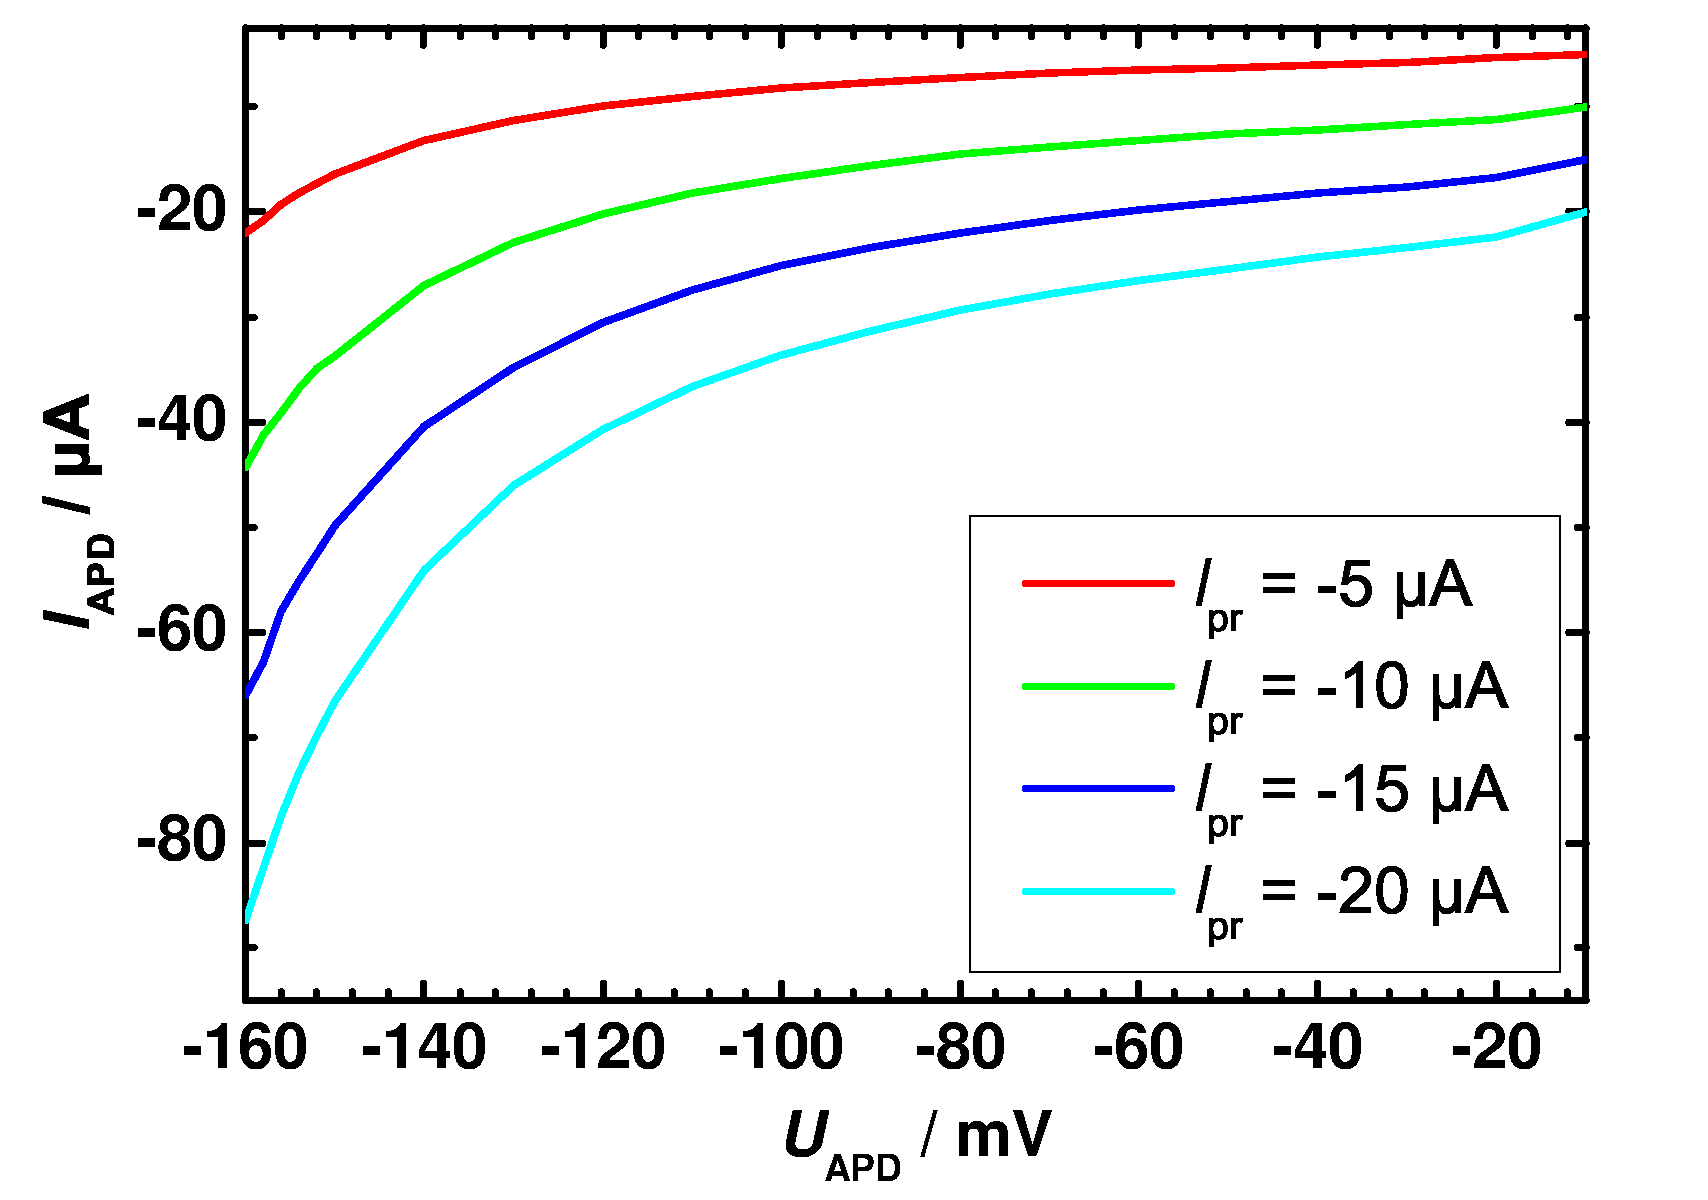
\includegraphics[width=.5\columnwidth]{Grafiken/T3_1.pdf}%
\caption{Relationship between  $I_{\mathrm{APD}}$,  $U_{\mathrm{APD}}$ and  $I_{\mathrm{pr}}$. }%
\label{fig:T3_1}%
\end{figure}

Figure \ref{fig:T3_1} shows the relationship between $I_{\mathrm{APD}}$,  $U_{\mathrm{APD}}$ and  $I_{\mathrm{pr}}$.
For $U_{\mathrm{APD}} < -120$~V the diode gets nonlinear. 

Figure \ref{fig:T3_2} shows the linear dependency of $I_{\mathrm{APD}}$ on $I_{\mathrm{pr}}$ for different voltages $U_{\mathrm{APD}}$ in the range of $-5~\upmu\mathrm{A} > I_{\mathrm{pr}} > - 20~\upmu\mathrm{A}$. With a higher voltage $U_{\mathrm{APD}}$ the slope gets steeper and the diode more sensitive.

\begin{figure}%
\centering
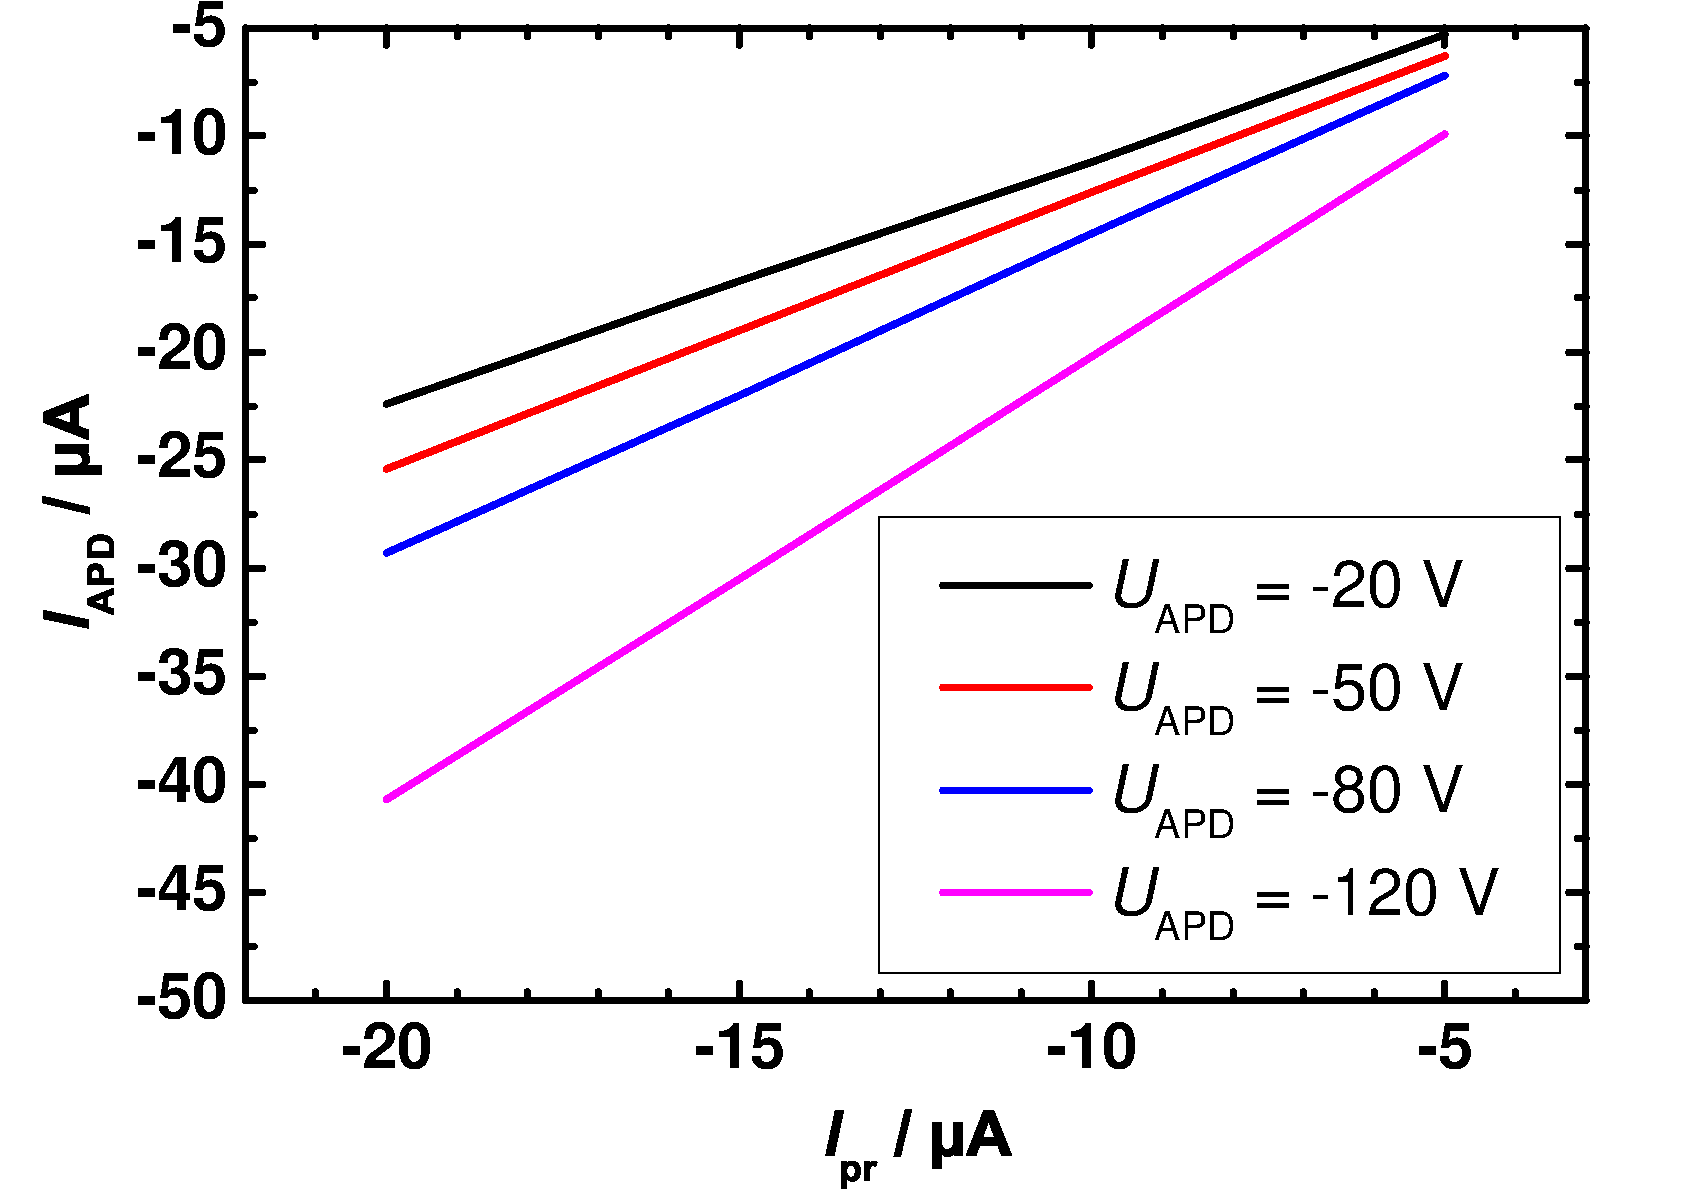
\includegraphics[width=.5\columnwidth]{Grafiken/T3_2.pdf}%
\caption{Linear dependency of $I_{\mathrm{APD}}$ on $I_{\mathrm{pr}}$ for different $U_{\mathrm{APD}}$.}%
\label{fig:T3_2}%
\end{figure}

The avalanche multiplication factor estimated by the formula

\begin{equation}
M_0(U_{\mathrm{APD}})=\frac{I_{\mathrm{APD}}(U_{\mathrm{APD}})}{I_{\mathrm{APD}}(U_{\mathrm{APD,min}}=-10\mathrm{~V})}.
\label{eq:M0}
\end{equation}

This function is plotted in figure \ref{fig:T3_3} for a primary photo current $I_{\mathrm{pr}}=-20~\upmu$A . To estimate the breakthrough voltage $U_{\mathrm{BR}}$ of the APD another formula\footnotemark[2] for $M_0$ was was used:
\begin{equation}
M_{\mathrm{th}} = \frac{1}{1-(U/U_{\mathrm{BR}})^n},
\label{eq:Mth}
\end{equation}
where $n$ is an adaption parameter. 
This function was fitted to the values of $M_0$. The resulting function is

\begin{equation}
M_{\mathrm{th}} = \frac{1}{1-(\frac{U}{-190~\mathrm{V}})^{1.44}},\qquad U_{\mathrm{BR}}=-190~\mathrm{V}
\label{eq:M_fit}
\end{equation}
which is also plotted in figure \ref{fig:T3_3}.
With that the breakthrough voltage can be estimated as -190~V.

\begin{figure}%
\centering
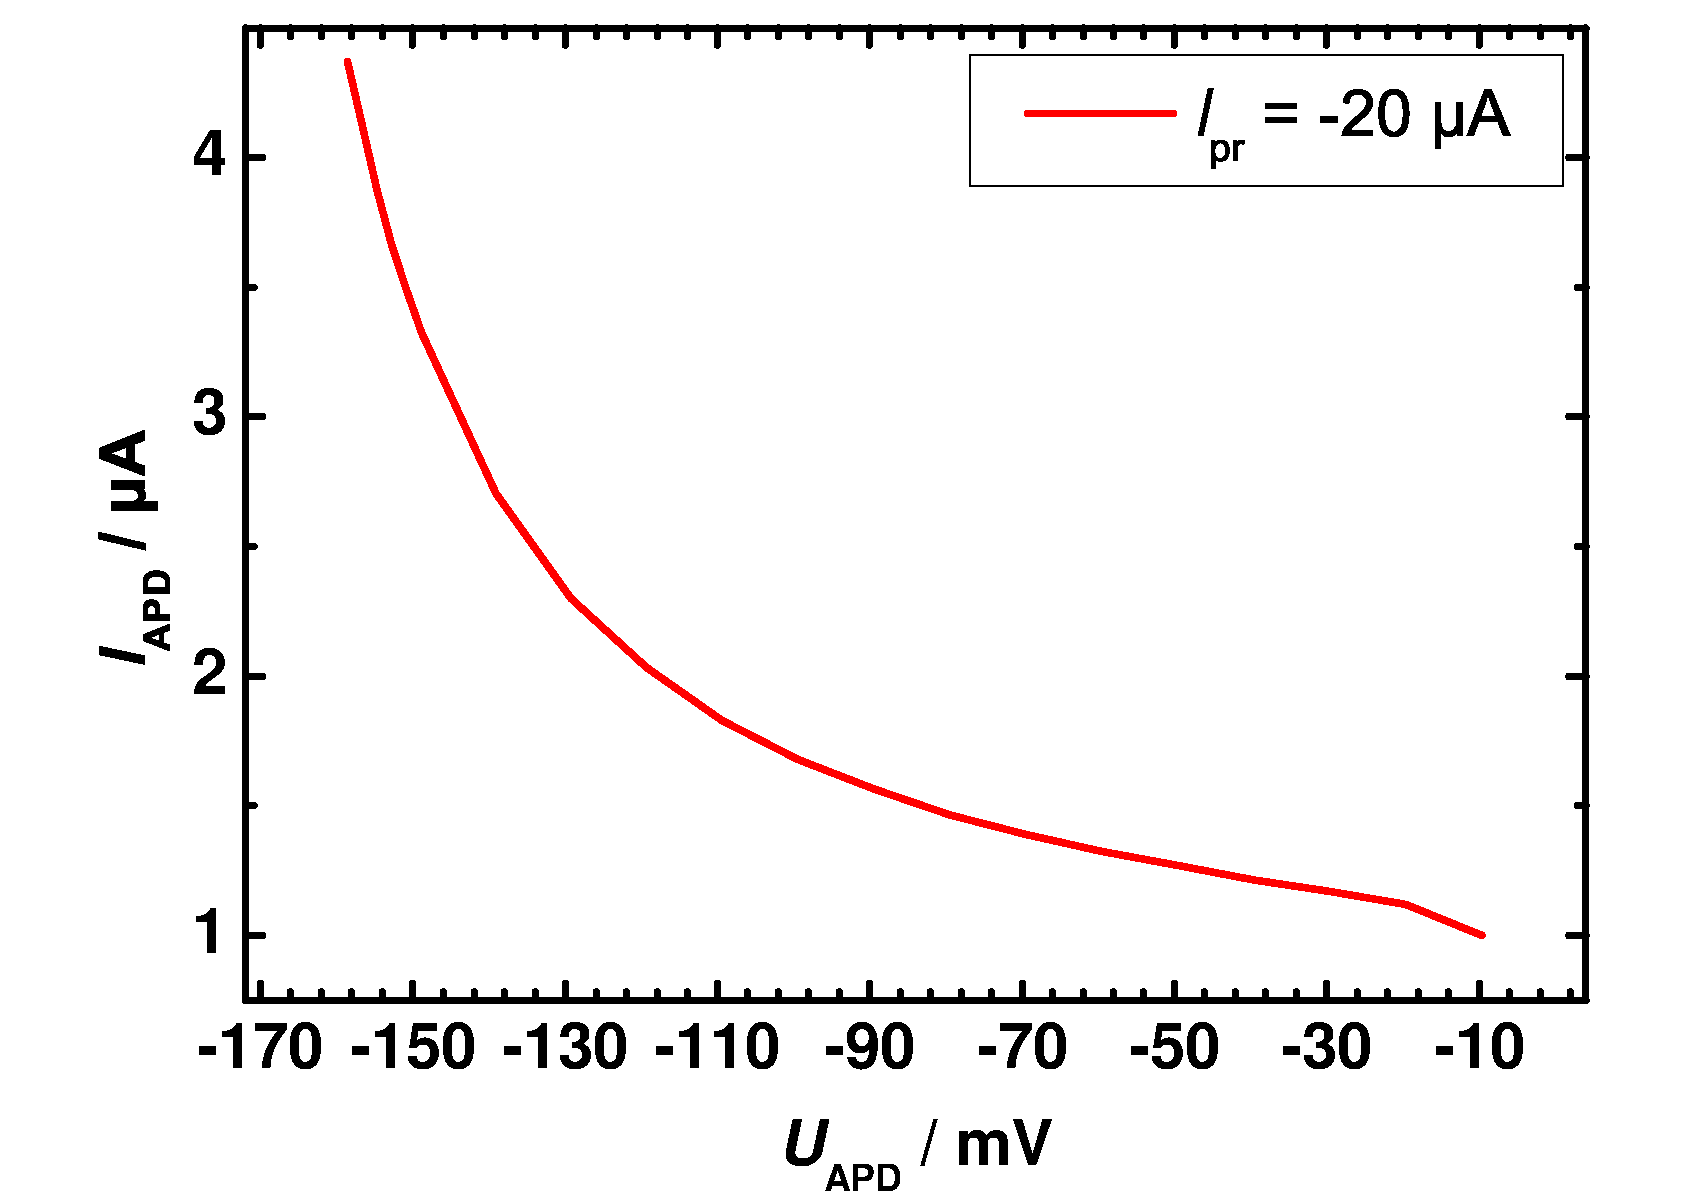
\includegraphics[width=.5\columnwidth]{Grafiken/T3_3.pdf}%
\caption{Calculated multiplication factor $M_0$ and theoretical multiplication factor $M_{\mathrm{th}}$ over $U_{\mathrm{APD}}$.}%
\label{fig:T3_3}%
\end{figure}